\subsection{Проектирование архитектуры ПО (модули)}

Архитектура программного обеспечения (англ. software architecture) - совокупность важнейших решений об организации программной системы.

Архитектура включает:

\begin{itemize}
    \item выбор структурных элементов и их интерфейсов, с помощью которых составлена система, а также их поведения в рамках сотрудничества структурных элементов
    \item соединение выбранных элементов структуры и поведения во всё более крупные системы
    \item архитектурный стиль, который направляет всю организацию - все элементы, их интерфейсы, их сотрудничество и их соединение.
\end{itemize}

Документирование архитектуры программного обеспечения (ПО) упрощает процесс коммуникации между разработчиками, позволяет зафиксировать принятые проектные решения и предоставить информацию о них эксплуатационному персоналу системы, повторно использовать компоненты и шаблоны проекта в других.

Архитектурный вид состоит из 2 компонентов:

\begin{enumerate}
    \item [1.] Элементы
    \item [2.] Отношения между элементами
\end{enumerate}

Архитектурные виды можно поделить на 3 основных типа:

\begin{itemize}
    \item [1.] Модульные виды (англ. module views) - показывают систему как структуру из различных программных блоков.
    \item [2.] Компоненты-и-коннекторы (англ. component-and-connector views) - показывают систему как структуру из параллельно запущенных элементов (компонентов) и способов их взаимодействия (коннекторов).
    \item [3.] Размещение (англ. allocation views) - показывает размещение элементов системы во внешних средах.
\end{itemize}

Примеры модульных видов:

Декомпозиция (англ. decomposition view) - состоит из модулей в контексте отношения <<является подмодулем>>.

Использование (англ. uses view) - состоит из модулей в контексте отношения <<использует>> (т.е. один модуль использует сервисы другого модуля).

Вид уровней (англ. layered view) - показывает структуру, в которой связанные по функциональности модули объединены в группы (уровни).

Вид классов/обобщений (англ. class/generalization view) - состоит из классов, связанные через отношения <<наследуется от>> и <<является экземпляром>>.

\subsubsection*{Иерархия модулей и подмодулей разрабатываемой программы}

Информационная система <<Товары>> включает в себя следующие модули:

\begin{itemize}
    \item Модуль организации локальной базы данных с выводом информации о товарах, включающий в себя меню
    \item Модуль, реализующий добавление новых записей в базу данных
    \item Модуль, осуществляющий сортировку записей в базе данных
    \item Модуль удаления записи/записей из локальной базы данных
    \item Модуль, осуществляющий поиск записи по реализованной базе данных
\end{itemize}

Некоторые модули являются подмодулями других, более общих модулей. Таким образом, в данной программе модули добавления, удаления, сортировки и поиска записи/записей будут являться подмодулями главного модуля, отвечающего за вывод локальной базы данных на экран с данными о спортсменах футбольной команды и организацией меню. Графически связь основного модуля с его подмодулями изображена на рисунке \ref{fig:modules} (рис. \pageref{fig:modules}).

\begin{figure}[!htp]
    \centering{
        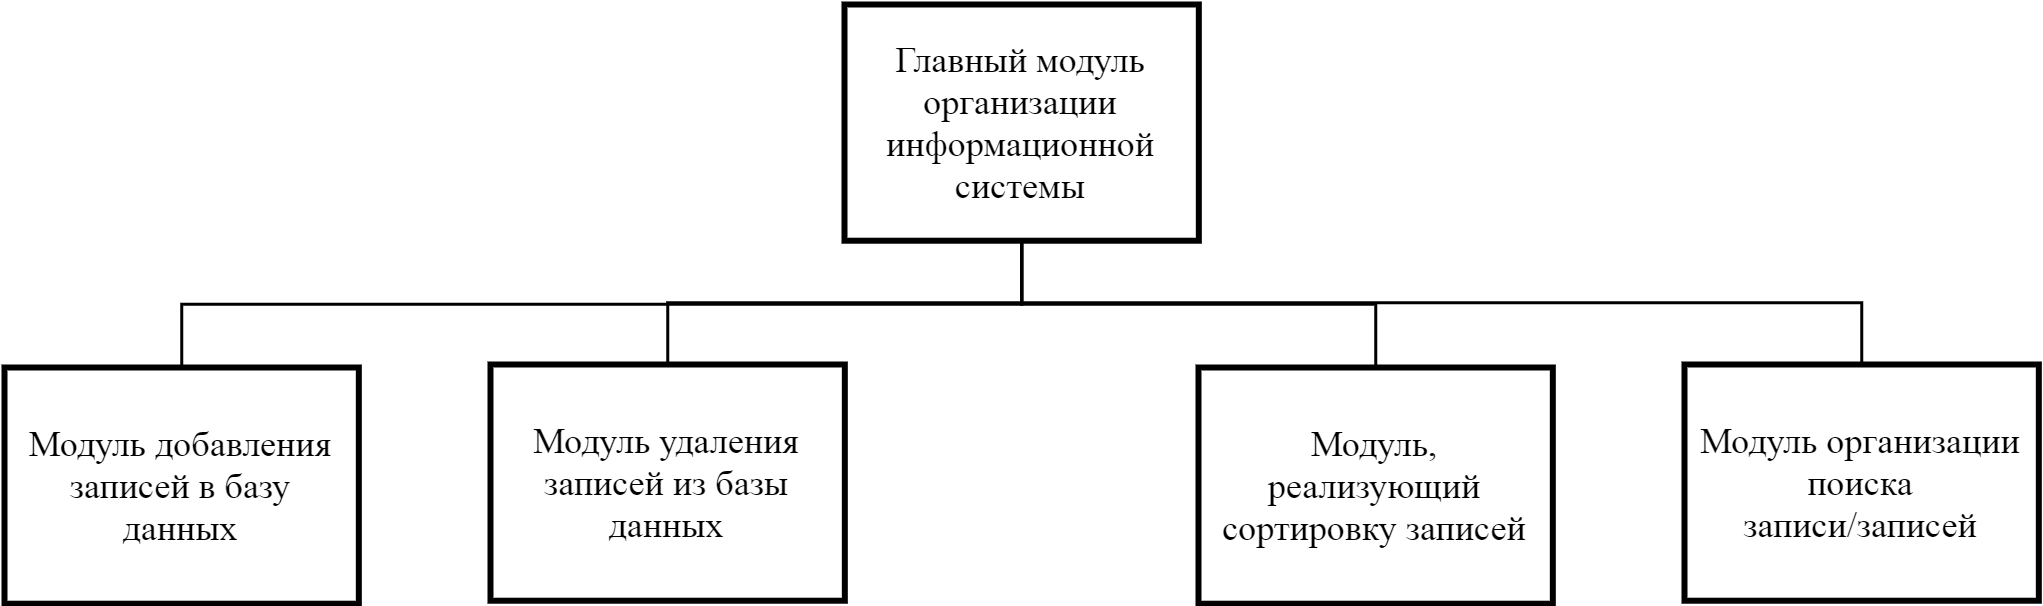
\includegraphics[]{../_input/formulationOfTheProblem/softwareArchitectureDesignModules/modules.png}
    }
    \caption{Модули и подмодули}
    \label{fig:modules}
\end{figure}
